 Web services are one of the main methods to provide utility computing. A definition for a web service is  
\begin{quote}A web service is a software system designed to support interoperable machine-to-machine interaction over a network. 
It has an interface described in a machine-processable format.\cite{webservdef}\end{quote}
They represent an easy way for developers and clients to access and compute information. Usually through an API users are
able to communicate with a web service although sometimes they need to be accessed with raw URL or HTTP request as seen in figure \ref{fig:webserv}.
Unlike traditional client/server models, such as a web server/web page system, web services do not provide the user with a GUI.
Instead they share business logic, data and processes through a programmatic interface across a network. The applications
interface, not the users. Developers can then add the web service to a GUI (such as a web page or an executable program) to offer
specific functionality to users.
\begin{figure}[htp]
\centering
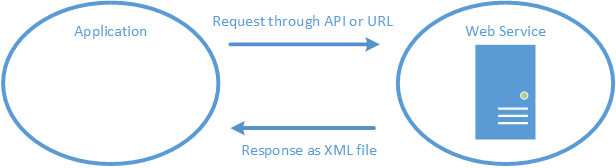
\includegraphics[scale=0.7]{Figures/WebService.png}
\caption{Simple diagram explaining how clients communicate with webservices}
\label{fig:webserv}
\end{figure}
Web services hold many benefits for developers. They represent components on the web that can be plugged in any project
or software so their functionality can be used. It improves communication between companies and users because information
is distributed much faster. A good example of a web service is of Google who provide an API to their GPS maps which when 
given longitude and latitude return a map with the location of the user.
\paragraph{}
A problem with web services are that if they go offline or they have a bug, they affect the whole network and every
application using them. Every non-open sourced framework is essentially a black box and the way it uses its parameters is unknown.
However these problems are minor to the overall benefit of the web services. Because of the way the internet works
the amount of web services has essentially created a distributed system with multiple components. Developers can integrate
complex systems easier than before and can easily plug in additional functionality as long as the right web service is there.


